\documentclass[../../../Bachelorarbeit.tex]{subfiles}
\begin{document}

\subsection{Vorstellung der Laboranlage}
In diesem Unterkapitel wird zunächst die Laboranlage vorgestellt, die im Verlauf der Arbeit unter den Gesichtspunkten des Requirements-Engineerings und der Anlagenprojektierung konzipiert, projektiert und in Betrieb genommen werden soll. Im ersten Abschnitt wird das bereits elektrisch fertiggestellte Positioniersystem dargestellt. Im Mittelpunkt steht hierbei die Erläuterung des Aufbaus und die Beschreibung der Funktionalität der Anlage. Der zweite Abschnitt behandelt die Eingliederung des Systems in seine Arbeitsumgebung. Dabei soll ein erster Überblick zum Einsatz der Positioniereinheit gegeben werden. Zuletzt werden die Betriebsmodi der Laboranlage vorgestellt, wobei genauer auf den Workflow im jeweiligen Modus eingegangen werden soll.

\subsubsection{Aufbau des Positioniersystems} \label{aufbau}
Wie bereits aus dem Thema der Bachelorthesis erkenntlich ist, handelt es sich bei der behandelten Laboranlage um ein mehrachsiges Positioniersystem. Dieses besitzt zum Zeitpunkt der ersten Inbetriebnahme zwei Achsen (siehe \autoref{fig:my-img60}).\\

\begin{figure}[H]
    \centering
    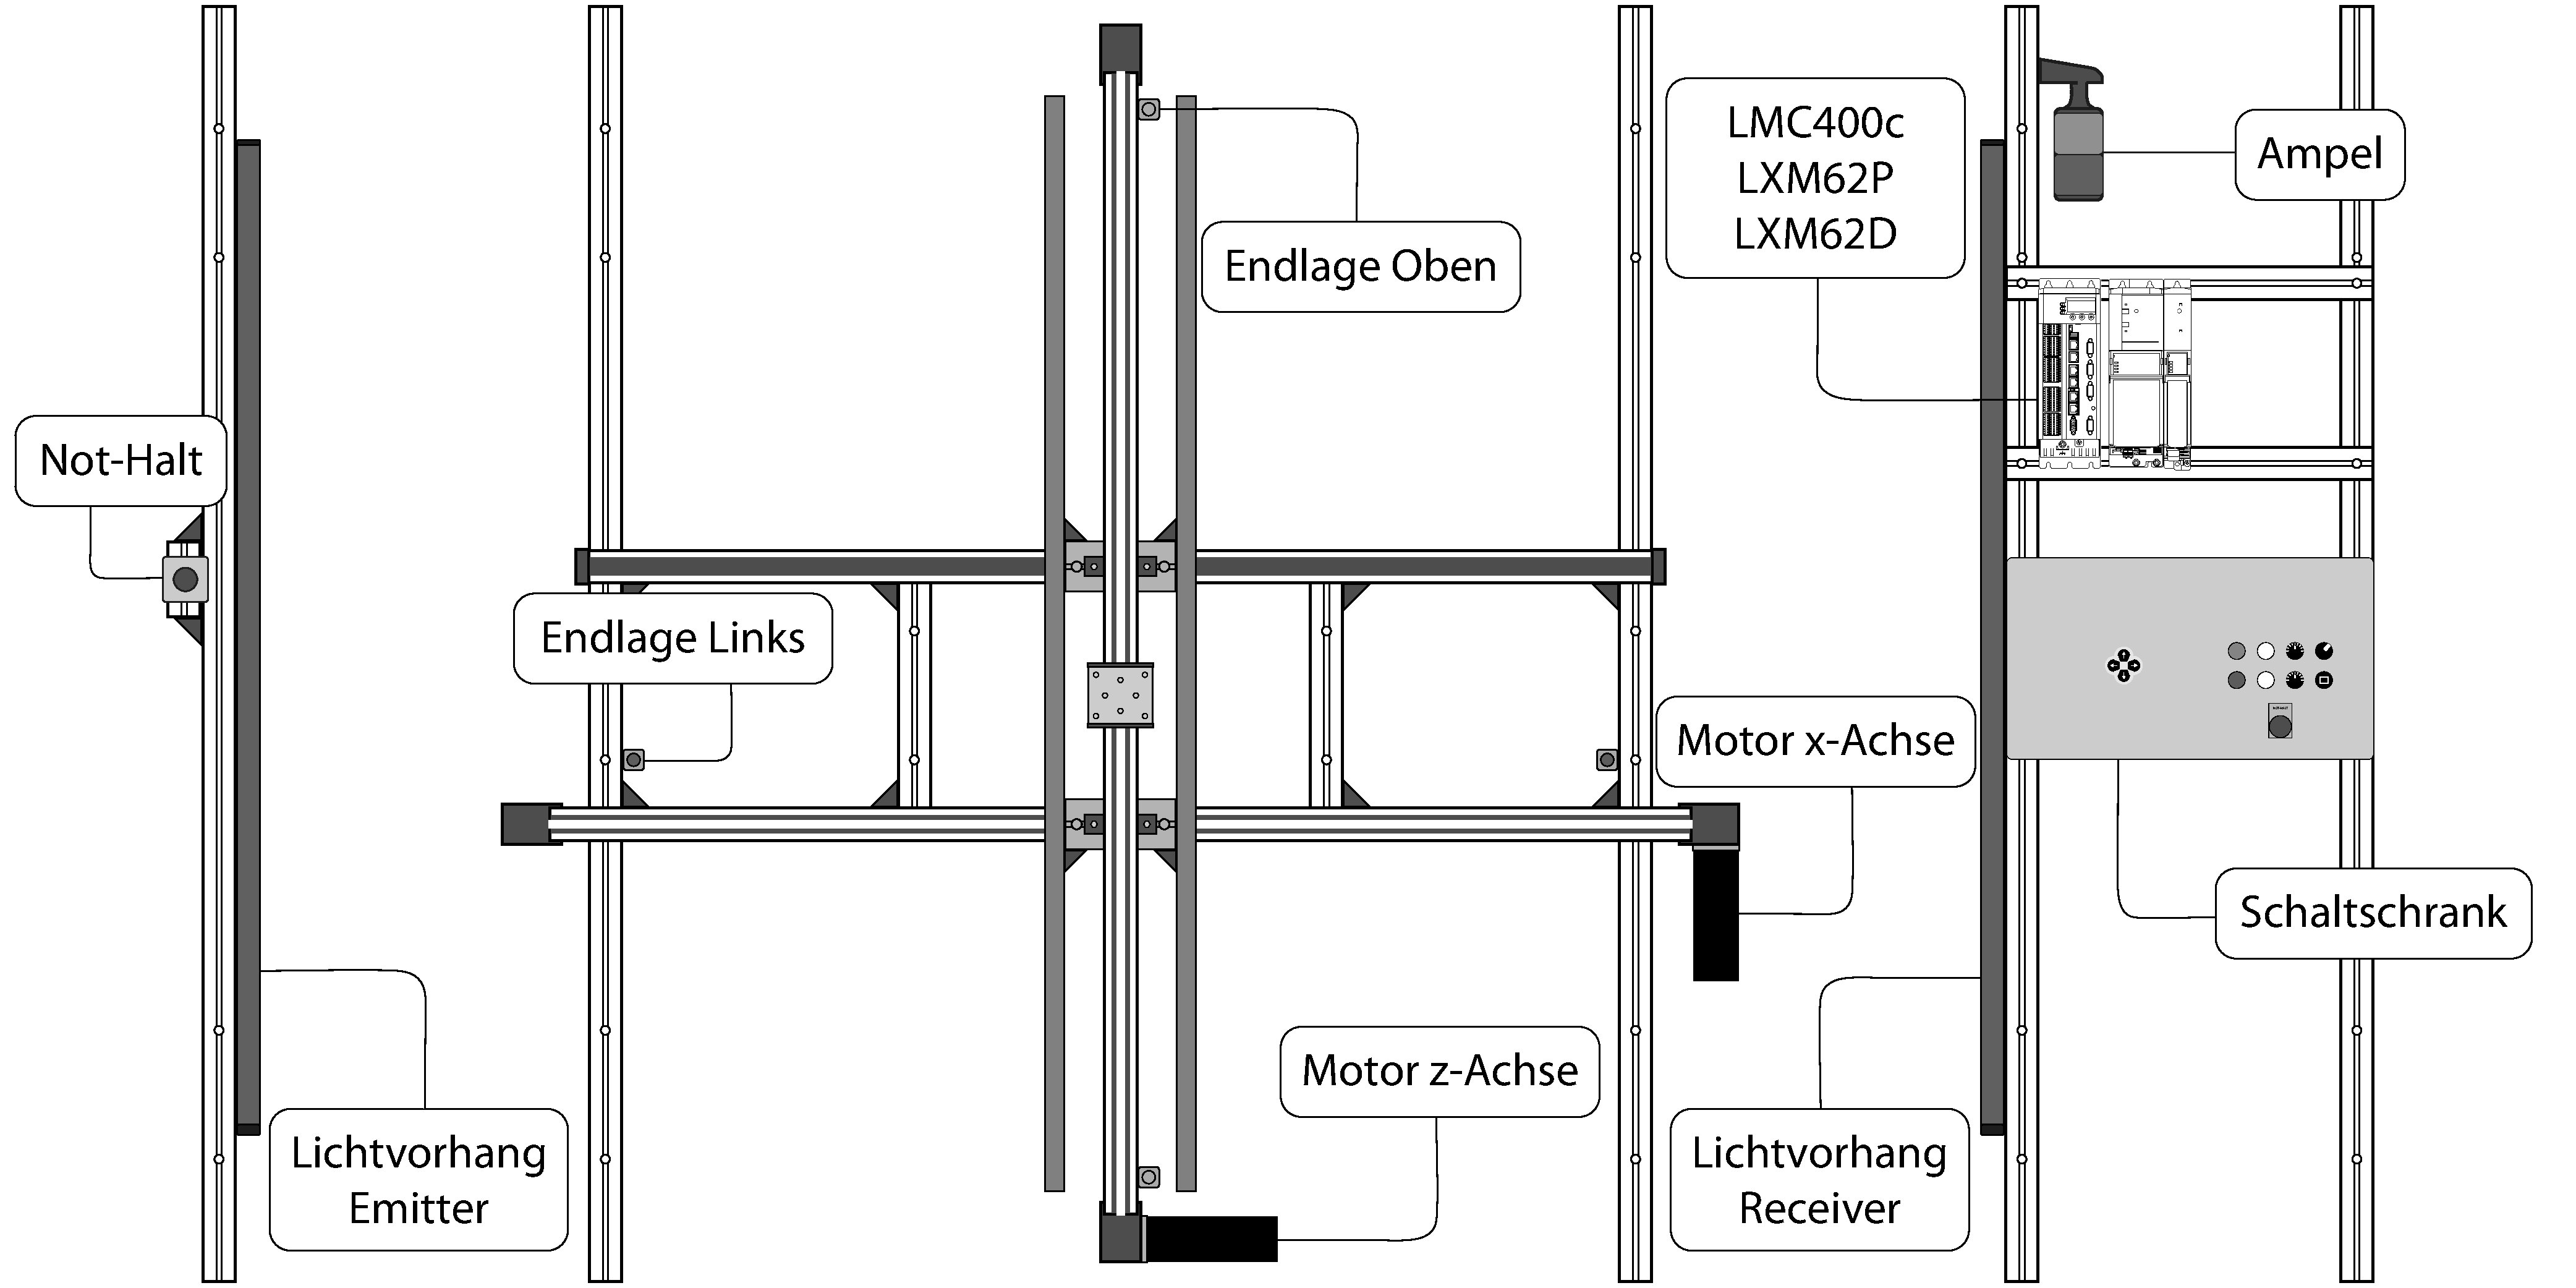
\includegraphics[width=\textwidth]{Images/konfigurator.pdf}
    \caption[Konfigurator]{Konfiguratorskizze des Positioniersystems}
    \label{fig:my-img60}
\end{figure}

Die horizontale Achse des Systems ist fest an der Wand montiert und hat eine Länge von rund 1600 \si{mm} (effektiver Fahrtweg). Vertikal montiert auf dieser befindet sich die beweglich gelagerte zweite Achse der Positioniereinheit. Diese besitzt die Möglichkeit, lineare Bewegungen zwischen den Endlagesensoren der Horizontalachse durchzuführen. Bei der Befestigung an der waagerechten Achse handelt es sich um ein doppeltes Schlittensystem auf Rollen. Die Bewegung der Achse erfolgt über ein Gummiriemen, der fest an der Vertikalachse befestigt ist, und über Umlenkrollen und einen Servomotor an der Horizontalachse bewegt werden kann. Auf der senkrechten Achse befindet sich ein weiterer Schlitten, der ebenso beweglich gelagert ist und sich auf einem Fahrtweg von rund 2000 \si{mm} zwischen zwei Endlagen bewegen kann. Auf diesem ist ein simples Greifsystem angebracht, welches horizontale 180 Grad Schwenkbewegungen durchführen kann und in der Lage ist, grundlegende Greifoperationen durchzuführen.\\
Für die Zuleitungen zu den auf den bewegten Anlagenteilen montierten Aktoren und Sensoren wurden Energieketten verbaut, sodass Kabel prozesssicher mitgeführt und eine dauerhafte Strom- sowie Datenversorgung aller Systemkomponenten gewährleistet werden kann. An den beiden äußersten Profilen (sowohl auf der linken als auch auf der rechten Seite der Anlage) sind Ablagepositionen vorgesehen, von \bzw auf welche simple Transportgüter aufgenommen und abgelegt werden können.\\
Auf der rechten Seite direkt neben der Positioniereinheit sind der Schaltschrank sowie die speicherprogrammierbare Steuerung (im Folgenden als \acs{sps} bezeichnet) an der Wand montiert. Die Kabel der Aktoren und Sensoren des Systems münden an der Unterseite des Schrankes sowie die Stromzuleitung und sämtliche Aus- und Eingangsverbindungen zu \bzw von der \acs{sps} und dem sich neben dieser befindenden Servoantrieb. Auf der Vorderseite an der Tür des Schaltschrankes sind Bedienelemente aufgeschraubt, die für die grundlegende Steuerung der Anlage benutzt werden können.\\
Zur Gewährleistung der Sicherheit von Mensch und Anlage sind am Eingang des Positioniersystems sowohl ein Lichtvorhang als auch Not-Halt Bedienelemente montiert. Stromfrei kann die Anlage über den Hauptschalter an der rechten Seite des Schaltschrankes geschaltet werden.

\subsubsection{Betriebsumgebung}
Nachdem im vorhergehenden Abschnitt bereits die grundlegenden Funktionen und der Aufbau der Positioniereinheit dargestellt wurden, beschäftigt sich dieses Unterkapitel mit der Darstellung der Eingliederung des Systems in dessen Arbeitsumgebung.\\
Aufgebaut befindet sich das mehrachsige Positioniersystem im Laborraum G422 der HTW Berlin am Campus Wilhelminenhofstraße. \autoref{fig:my-img61} zeigt das Gehäuse/Gerüst des Positioniersystems an der Rückwand des Laborraumes. Dort wurde die Laboranlage im Rahmen meines Praktikums errichtet. Nachfolgen ist es Ziel der Bachelorthesis, diese Anlage für den Lehrzweck in Betrieb zu nehmen. Konkret soll die Positioniereinheit für zwei Anwendungen eingesetzt werden.\\

\begin{figure}[H]
    \centering
    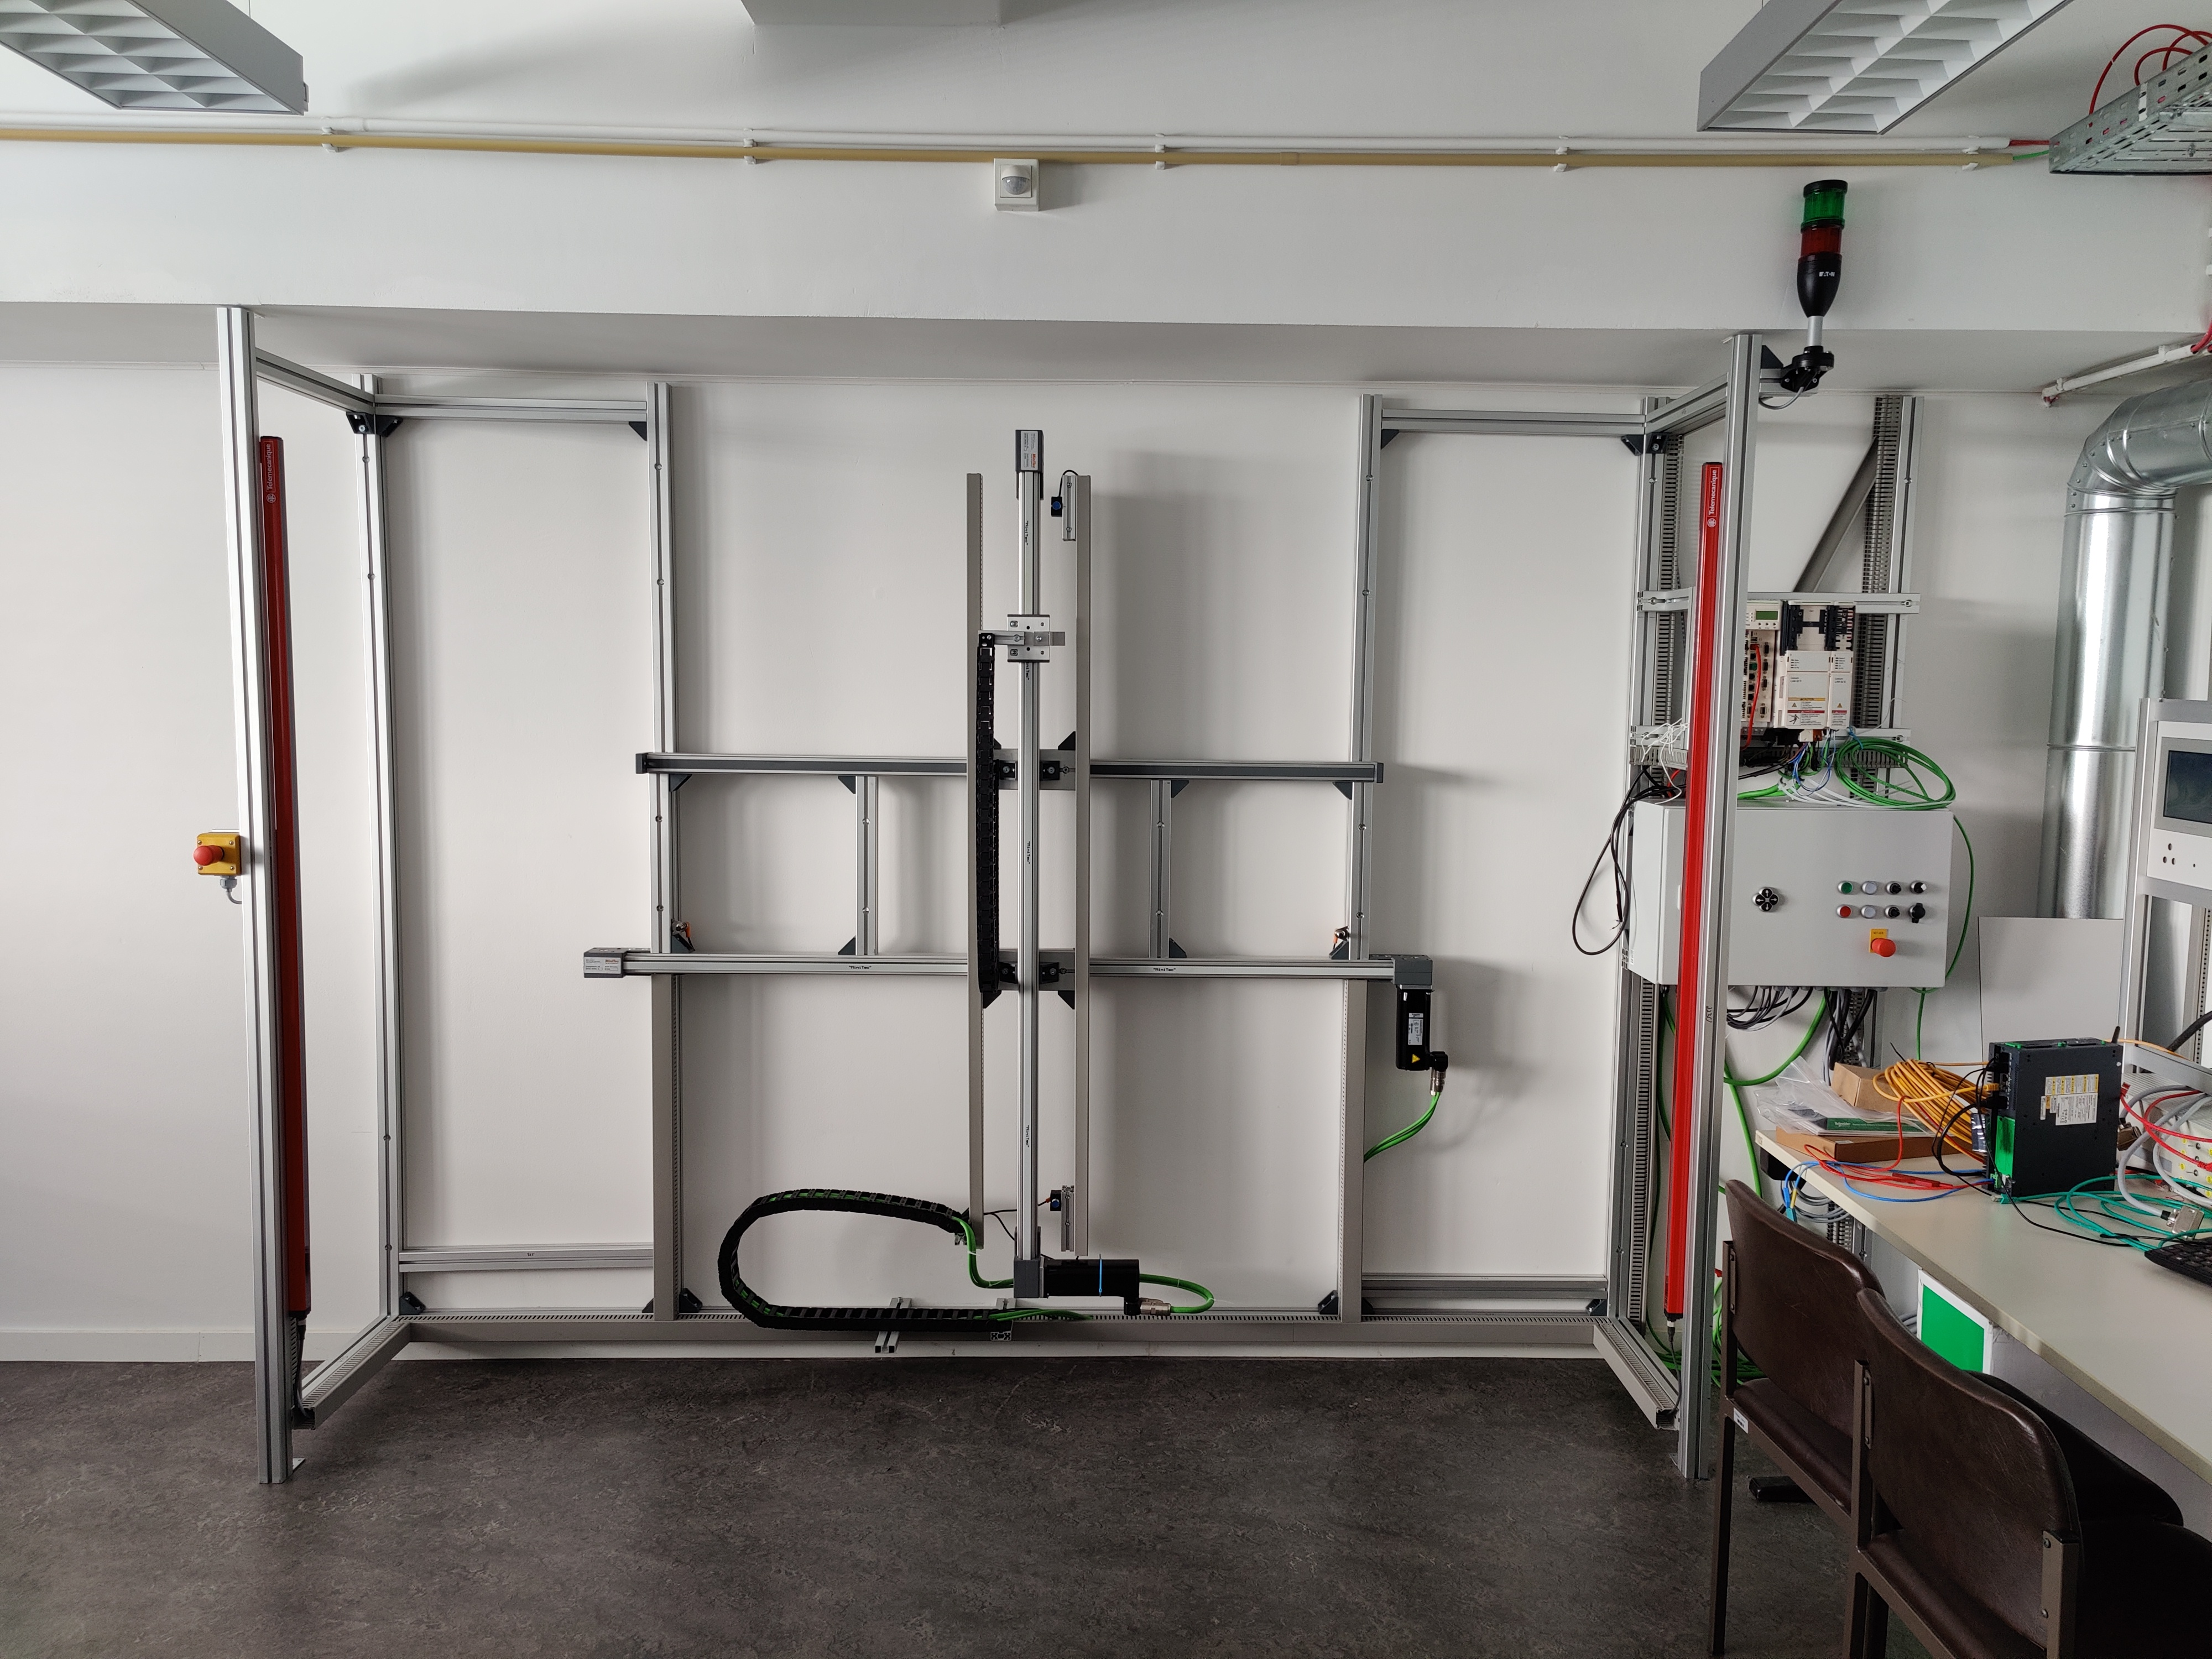
\includegraphics[width=0.7\textwidth]{Images/laborraum.jpg}
    \caption[Laborraum]{Reale Anlage im Laborraum G422 an der HTW Berlin Campus Wilhelminenhofstraße}
    \label{fig:my-img61}
\end{figure}

Erstere gliedert sich direkt in die Unterrichtseinheiten des Laborbetriebs im späten Bachelor- und das gesamte Masterstudium im Themenfeld Automatisierungstechnik ein. Jeder studentische Laborplatz besitzt die Möglichkeit, sich mit dem System zu verbinden, um es mit Automatisierungssoftware, die in den Lehreinheiten entwickelt wird, zu bespielen und diese an der Anlage zu testen. Es soll die Möglichkeit bestehen, Trajektorien zu fahren, bei denen virtuelle Hindernisse umgangen werden und Objekte von einem Ausgangspunkt zu einem Zielpunkt transportiert werden können. Die Nutzung der realen Anlage dient dabei als Prüfmöglichkeit der vorher von den Studierenden nur simulativ getesteten Automatisierungssoftware. Ziel ist es, den Laboranten eine Laboranlage zur Verfügung zu stellen, die in der Industrie in ähnlicher Weise aufzufinden ist, um bereits im Studium spätere Arbeitsabläufe aufzuzeigen.\\
Die zweite Anwendung des mehrachsigen Positioniersystems ist Teil eines laborübergreifenden Projektes, welches nicht in dieser Arbeit behandelt wird. Aus dessen Zielen ergeben sich weitere Anforderungen an die Laboranlage. Es sollen Daten aus dem Prozessablauf bereitgestellt werden, aus denen eine Wertschöpfung für das Projekt generiert werden kann. Die gewonnenen Daten sollen extern weiterverarbeitet werden. Dazu müssen weitere Schnittstellen im System bereitgestellt werden, um generierte Daten mit Peripheriegeräten austauschen zu können.

\subsubsection{Vernetzung des Systems}
Das Positioniersystem ist in das Labornetzwerk des Raumes eingebunden. Im selben Netzwerk befinden sich sämtliche Computer der einzelnen Arbeitsplätze. Verbunden sind das Positioniersystem und die Laborrechner über drei Internetswitches im selben Raum. Das mehrachsige Positioniersystem verfügt intern über einen weiteren Switch, über den die beiden Steuerungen des Systems mit dem Labornetzwerk verbunden sind. Die \acs{ea}-Module und die Sicherheitssteuerung im Schaltschrank sind über den SERCOS-III-Bus mit der Hauptsteuerung (\acs{lmc}400c) des Systems verbunden. Weitere Busteilnehmer sind das Netzteil und der Servoregler. \autoref{fig:my-img62} zeigt die beschriebene Netzwerkstruktur.

\begin{figure}[H]
    \centering
    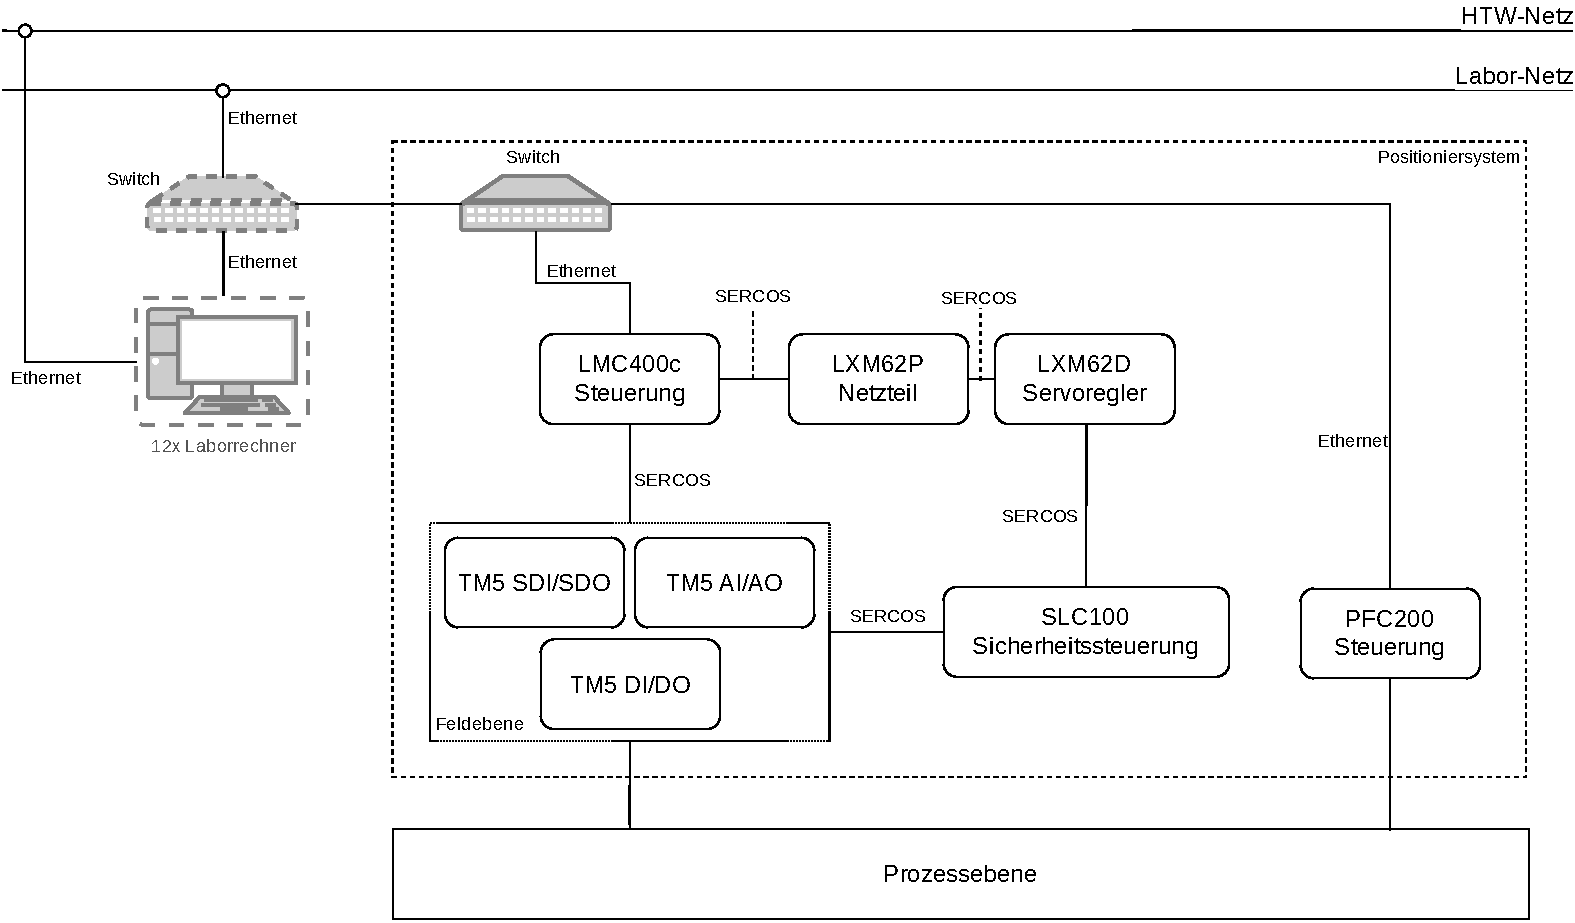
\includegraphics[width=\textwidth]{Images/Netzwerkdiagramm.pdf}
    \caption[Netzwerkstruktur]{Netzwerkdiagramm - Vernetzung des mehrachsigen Positioniersystems}
    \label{fig:my-img62}
\end{figure}

% TODO: Übersichtsgrafik Betriebsmodi einfügen
\subsubsection{Betriebsmodi}
Die Nutzung der Laboranlage erfolgt in zwei verschiedenen Betriebsmodi. Um den Produktivbetrieb des Positioniersystems einzuleiten, muss der Nutzer zwischen dem Automatikmodus und dem Handmodus auswählen, die im Folgenden detailliert beschrieben werden.
\bigskip
\newline
\textbf{Automatikbetrieb:} Bei dem Automatikmodus handelt es sich um den üblicherweise genutzten Betriebsmodus der Laboranlage. Dieser kann vollautomatisch im Dauerbetrieb eingesetzt werden und erfordert nicht die Anwesenheit vom Nutzer. Der Prozessablauf ist programmatisch vorgeschrieben und wird zyklisch durchgeführt. Zur erstmaligen Inbetriebnahme sollen einfache Transportaufgaben durchgeführt werden. So könnte beispielsweise von einer Ablageposition A ein Transportobjekt gegriffen und um Hindernisse herum transportiert werden, sodass besagtes Objekt an einer Zielposition B wieder abgesetzt wird. Danach fährt die Anlage wieder zu Position A, um erneut ein Objekt für den Transport aufzunehmen.\\
Konkret muss das Positioniersystem im ersten Schritt unter Spannung gesetzt, in dem der Hauptschalter (400 \si{V} Ebene) betätigt wird. Dieser befindet sich, wie bereits im vorherigen Unterkapitel erwähnt, auf der rechten Seite des Schaltschrankes. Darauffolgend muss im zweiten Schritt die Steuerung (\acs{lmc}400c von Schneider Electric) eingeschalten sowie alle Betriebsmittel auf der 24 \si{V} Ebene mit Strom versorgt werden. Dies geschieht über einen Leitungsschutzschalter im Schaltschrank. Der eingeschaltete Zustand ist am grünen Leuchten der Status-LED des \acs{lmc} zu erkennen. Als Netzteil dient das \acs{lxm}62 P Powersupply von Schneider Electric, welches 3-phasig an der Drehstromsteckdose des Laborraumes angeschlossen ist. Dieses versorgt den LXM 62D double Drive aus der gleichen Produktreihe wie das Netzteil. Die 24 \si{V} Steuerungsebene wird aus einer separaten Steckdose versorgt. Mit einem Wahlschalter kann nun der Automatikmodus des Systems angewählt werden. Bestätigt wird dieser über den Start-Taster an der Schaltschranktür. Die erfolgreiche Auswahl des Automatikmodus kann an der Signalampel des Systems abgelesen werden (zweifarbiges Blinken). Die Anlage wechselt aus dem Leerlauf in den vollautomatischen Betrieb.\\ 
Nach der Wahl des Automatikmodus bewegt das Positioniersystem die auf den beiden Achsen montierte Greifeinrichtung aus der Ausgangsposition des Leerlaufes (auch als Home bezeichnet) zur Ablageposition A. Dazu werden zunächst die Bremsen der beiden Motoren gelöst, welche für die Bewegung der jeweiligen Achse verantwortlich sind. Ist die Position vor der Ablageposition A erreicht, wird im nächsten Schritt ein Schwenkarm mit Greifer so zur Ablageposition A rotiert, dass ein sich darauf befindliches Objekt gegriffen werden kann. Es folgt besagter Greifprozess, um das auf Ablageposition A befindliche Objekt aufzunehmen.\\
Das Positioniersystem muss nun einen Fahrtweg bewältigen, der mit virtuellen Hindernissen bestückt ist, um Trajektorien zum Transport von Gütern in mit Objekten blockierten Umgebungen zu erproben. Es ist nicht möglich, eine geradlinige Bewegung von Startposition A zur Zielposition, dem Ablageort B, zu fahren. Weiterhin kann auch nicht erst der komplette Fahrtweg in vertikaler Richtung (z-Richtung) bewältigt werden und dann die Bewegung in horizontaler Richtung (z-Richtung), noch eine geradlinige Bewegung, sodass die z- und x-Koordinate des Zieles gleichzeitig erreicht werden. Die Hindernisse werden programmatisch vorgegeben und sind somit der Laboranlage \bzw der Automatisierungssoftware bekannt.\\
im nächsten Schritt werden dem Positioniersystem Koordinaten übergeben, die, wenn diese durchfahren werden, den Weg von Startposition A zu Zielposition B ergeben. Dabei soll berücksichtigt werden, dass nur an der Start- und Zielposition umfangreichere Beschleunigungen stattfinden sollen, welche die Achsen aus der Ruhe beschleunigen \bzw diese wieder abbremsen, die einzelnen Punkte auf dem Weg werden nur durchfahren. Zur Minimierung von starken Trägheitsmomenten ist es weiterhin notwendig, dass die beiden Achsen zusammen keine gradlinigen Fahrtwege zwischen den Wegpunkten nutzen, sondern in abgerundeten (gedämpften) Trajektorien die einzelnen Koordinatenpunkte abfahren. Die konkrete Parametrierung der Fahrwegabschnitte und der sich daraus ergebenden Trajektoriemuster soll Teil der Testszenarien des mehrachsigen Positioniersystems sein.\\
An der Zielposition angekommen, schwenkt der sich auf der z-Achse befindende Arm um, und das Objekt wird über der Ablageposition vom Greifer losgelassen, sodass es auf der Zielposition verweilt. Die Anlage fährt nun den Weg zur Startposition zurück, um ein weiteres Objekt aufzunehmen und dieses wie bereits beschrieben zu transportieren.\\
Mögliche spätere Erweiterungen könnten sein, dass der Rückweg anders gewählt wird, da kein Objekt transportiert wird und somit auftretende Trägheitsmomente und Schwingungen keine wichtige Rolle spielen. Alternativ könnte auch auf dem Rückweg ein anderes Objekt von Ablageposition B zu Ablageposition A transportiert werden, welches andere Eigenschaften aufweist, was den Fahrtweg beeinflussen könnte.\\
Für die vollständige Automatisierung des Prozesses ist eine spätere Erweiterung nötig, bei der auch die Ablageposition(en) automatisch mit neuen Transportobjekten bestückt werden. Es würde sich eine Aufrüstung mit Förderbändern von und zu den Ablagepositionen der Anlage lohnen, sodass steig neue Objekte dem Positioniersystem bereitgestellt und von diesem auch wieder entnommen werden können.\\
im letzten Schritt kann die Anlage wieder deaktiviert werden, was über die Abwahl des aktuellen Betriebsmodus geschieht. Es muss der gleiche Taster wie bei der Auswahl des Modus betätigt werden. Dies ist in jedem Moment während der Laufzeit des Automatikmodus möglich. Die letzte Transportaufgabe wird noch vollständig zu Ende durchgeführt. Danach findet das Homing statt, bei dem der sichere Ausgangszustand der Anlage wieder angefahren und die Bremsen der Motoren wieder aktiviert werden. Die Bremsen dienen beim Erreichen des Leerlaufes nicht nur zum Abbremsen der Achsen, sondern sind nötig, damit der Schlitten auf der Vertikalachse nicht bis nach unten fällt. Nach erfolgreicher Abwahl des Betriebsmodus erlischt die Indikatorlampe für den Automatikbetrieb wieder. Nur wenn kein Modus ausgewählt ist, kann die 24 V Ebene wieder spannungsfrei geschalten und die Laboranlage wieder deaktiviert werden. Dies geschieht über den Aus-Taster auf der Front des Schaltschrankes. Nach Betätigung des Tasters erlischt die Lampe, welche die Betriebsbereitschaft des Positioniersystems signalisiert.\\
% Während der gesamten Betriebsdauer gelten mehrere Safety-Bedingungen. Es befinden sich mehrere Not-Aus Taster (einrastend) an der Anlage (am Schaltschrank, auf der Linken Seite an einem Profil). Die Betätigung führt zu einem sofortigem halt der Bewegung beider Achsen und dem Anzug der Bremsen in den Motoren. Gleiche Funktionalität tritt auf, wenn der Lichtvorhang von einem Objekt (menschlich oder nicht menschlich) durchbrochen wird. Nach Auftreten dieses Ereignis muss die Anlage wieder freigeschalten werden. Der aktuelle Betriebsmodus wird abgewählt, was dafür sorgt, dass die Anlage im Fall des Automatikmodus nun den letzten bearbeitungsschritt fertig zu Ende durchführt und dann in die Ausgangsposition fährt. Alternativ kann auch der Admin-Modus aktiviert werden, um die letzte Aufgabe zu unterbrechen/beenden und das Positioniersystem manuell zu bedienen.\\
% Weiterhin muss während der gesamten Betriebsdauer eine Achsbewegung innerhalb der magnetischen Näherungssensoren gegeben sein. Wird eine Endlageposition auf einer der beiden Achsen überschritten, wird umgehend die Bremse des Motors der jeweiligen Achse aktiviert, so dass diese nicht über die Endposition hinausfahren kann und Beschädigungen verursacht. Da es sich bei der Bewegung der Achsen um eine geregelte Bewegung über Servos handelt kann davon ausgegangen werden, dass es sich bei der Aktivierung der Näherungsschalter um einen fehlerhaften Zustand handelt. Es wird analog zu der Not-Halt Funktionalität im vorhergehenden Absatz gehandelt.\\
% Als letztes wird noch die rote und grüne Ampel/Signalsäule erläutert, welche rechts oben an einem Profil der Anlage befestigt ist. Diese dient zur Signalisierung des Betriebes der Anlage. Sobald sich eine Achse in Bewegung befindet, blinkt die Ampel. Dies dient als Warnung für umstehende Menschen, dass diese sich im Bereich der Anlage vorsichtig und achtsam verhalten sollten. Im Fehlerfall leuchtet die Ampel in ausschließlich roter Farbe, ist die Positioniereinheit betriebsbereit, leuchtet sie nur in grüner Farbe.\\
% Weiterhin muss zu jedem Zeitpunkt, wo keine Bewegung einer Achse stattfindet die Bremse der jeweiligen Achse aktiviert sein.
\smallskip
\newline
\textbf{Handbetrieb:} Bei dem Handmodus handelt es sich um die zweite Betriebsart der Positioniereinheit. Anders als im Automatikbetrieb dient der Handmodus nicht als Abarbeitungsmodus für Positionieraufgaben, sondern soll als manuelle Bedienmöglichkeit genutzt werden können. Das heißt konkret, dass erst durch das Betätigen von Tastern Bewegungen und Aktionen durchgeführt werden.\\
Wie auch schon im Automatikmodus wird die Anlage zunächst unter Spannung gesetzt durch Betätigung des Hauptschalters. Anschließend fahren die Steuerungen hoch. Zur Auswahl des Handbetriebes muss nur der Betriebsmodusschalter auf \glqq HAND\grqq{} eingestellt und nachfolgend per Taster bestätigt werden. Die erfolgreiche Auswahl wird durch das Aufleuchten der weißen Taster an der Front des Schaltschrankes signalisiert.\\
Nach der Wahl des Handmodus verbleibt die Anlage zunächst im Ruhezustand. Die beiden Achsen befinden sich an der Ausgangsposition, die im Leerlauf aktuell gegeben ist. Um die Positioniereinheit in Bewegung zu setzen, ist nun eine Nutzereingabe nötig.\\
An der Frontseite des Schaltschrankes befindet sich ein Vierfachtaster mit Pfeilen in x- und z-Richtung. Mittels der Taster kann per Druck die jeweilige Achse bewegt (gejoggt) werden. Dies geschieht so lange, bis der Taster wieder losgelassen wird oder eine der Endlagen erreicht ist. Bei Betätigung eines Tasters fahren die Achsen jedoch nicht mit voller Geschwindigkeit an, sondern beschleunigen erst langsam. Auch die Beschleunigung beim Loslassen \bzw Abbremsen einer Achse ist verringert gegenüber dem Automatikmodus. Über zwei Potentiometer rechts neben den vier Bewegungstastern kann die Fahrtgeschwindigkeit reguliert werden.\\
Nach manuellem Navigieren zu den Ablagepositionen besteht an diesen die Möglichkeit, den Greifer einzusetzen. Nun muss jedoch jeder einzelne Schritt, also Umschwenken zur Ablage, Greifen und wieder Loslassen eines Transportobjektes per Druckknopf getriggert werden.\\
Weiterhin ist als Randbedingung im Handbetrieb vorgesehen, dass in den äußeren Bereichen des Positioniersystems zum einen nur geringere Geschwindigkeiten gefahren werden können als auch, dass die Beschleunigung der Achsen in diesen Bereichen gedämpft ist, um zu verhindern, dass die Schlitten auf den jeweiligen Achsen über die Endlagen hinaus Abbremsen und mit den harten Stoppelementen am äußersten Ende der Achsen kollidieren.\\
Im Handmodus sind keine virtuellen Hindernisse vorgesehen auf dem Fahrtweg des Greifers, da kein Mehrwert aus dem manuellen Umfahren gewonnen wird und maximal die Koordination des Nutzers trainiert werden kann. Programmatisch wäre an dieser Stelle kein Mehrwert zu erreichen, falls der Nutzer per Tastendruck Kollisionen mit Hindernissen verhindern sollte.\\
Nach Wiederabwahl des Handmodus durch den Stop-Taster ist die Anlage wieder im Leerlauf.
% Anders als im nächsten Kapitel beschrieben, kommt nun der Vierwegeschalter als Eingabegerät für bestimmte Anlagenfunktionalitäten zum Einsatz. Dieser ist beim Handbetrieb keine direkte Steuerung, um das auf den beiden Achsen montierte Greifgerät in die jeweilige Richtung der Pfeile auf den Tastern zu bewegen, sondern eine Eingabemöglichkeit, um das Positioniersystem zwischen den einzelnen Ablaufzuständen wechseln zu lassen.\\
% Die Taster mit den Pfeilen nach rechts und links veranlassen die Anlage zu einer Bewegung zum jeweils nächsten bzw. vorherigen Koordinatenpunkt im Funktionsablauf. Die Taster mit den Pfeilen nach oben und unten sind für die separate Steuerung des Greifers verantwortlich, welcher auf dem Schlitten der Z-Achse befestigt ist. Zum besseren Verständnis wird nun der Ablauf bzw. die Aufgabe, die auch schon im Kapitel zum Automatikbetrieb beschrieben wurde, analog nun für den Handbetrieb erläutert.\\
% Durch Drücken der Pfeiltaste nach rechts fährt die Anlage mit den beiden Achsen den Greifer aus der Ausgangslage zur Ablageposition A. Dort kann der Nutzer nun durch Betätigung des oberen Tasters der Vierwegeeingabeeinheit den Schwenkarm mit dem Greifer über die Ablageposition drehen lassen. Durch erneutes Drücken würde sich der Arm um 180° drehen, um eine Greifaktion auf der anderen Seite durchführen zu können. Um ein Objekt aus der Ablageschale aufheben zu können ist nun die Eingabe des Tasters mit dem Pfeil nach unten nötig. Erneutes Betätigen würde den Greifer wieder öffnen, um das gegriffene Objekt wieder entlassen.\\
% Genauso wie im Automatikbetrieb kann die Anlage keinen geradlinigen Weg zur Zielposition fahren, um das aufgenommene Objekt zu seiner Ablageposition zu bringen. Das Automatisierungsprogramm besitz wieder Informationen zu Bereichen, in denen sich Hindernisse befinden, die umfahren werden müssen. Anders jedoch als im Automatikmodus wird nun kein kompletter weg übermittelt, sondern nur einzelne Splines aus denen der Gesamtweg besteht. Somit wird jedes Hindernis einzeln umfahren, wenn es eine Wegkorrektur erfordert. Um eine Bewegung zu fahren muss der Nutzer mit der Pfeil nach rechts Taste die Anlage in Bewegung versetzen. Durch Drücken der linken Taste kann eine Bewegung rückgängig gemacht werden. Dass heißt die Anlage kann die bereits durchgeführten Fahrtwege umgekehrt wieder zurückfahren.\\
% Je nach Menge und Position der Hindernisse wird nach einigen Eingaben des Nutzers der Zielort erreicht. Dort kann durch die obere bzw. untere Taste des Vierwegeschalters das transportierte Objekt abgelegt werden. Durch weiteres Interagieren mit der Vorwärts-Taste fährt die Positioniereinheit den Greifer wieder zur Aufnahmeposition A.\\
% Beim Abwählen bzw. Deaktivieren des Handbetriebes ist es nicht vom Nutzer erforderlich, dass dieser die aktuelle Aufgabe händisch fertigstellt. Anstelle dessen fährt die Anlage direkt in den Ausgangszustand und aktiviert die Bremsen in den beiden Motoren. Zu jeder Zeit während des Betriebsablaufes im Handmodus kann auf den Automatikbetrieb umgeschaltet werden, was das Positioniersystem am aktuell vorliegenden Zustand ansetzen lässt, und von dort den Ablauf automatisch durchführt. Ab diesem Zeitpunkt gelten alle Regularien des Automatikbetriebes.\\
% Die Safety-Funktionen des Handbetriebes sind annähernd identisch zu denen des Automatikmodus. Bei Betätigung eines Not-Aus Tasters oder durchbrechen des Lichtvorhangs stoppt die Positioniereinheit direkt alle Bewegungen und aktiviert die Bremsen in den Motoren. Gleiches geschieht auch bei Überschreitung der Endlagen der jeweiligen Achsen. Nach wieder Freigabe beendet die Anlage den aktuellen Teilschritt des Prozessablaufes und geht somit in den nächsten Zustand über. Von dort kann der Nutzer mit dem Handbetrieb fortfahren. Es ist nicht erforderlich den Betriebsmodus zur Freischaltung abzuwählen oder auf den Admin-Betrieb zu wechseln. (Die Möglichkeit besteht wie zu jedem anderen Zeitpunkt dennoch.)\\
% Die Signalampel verhält sich wie im Automatikbetrieb, mit dem Zusatz, dass sie auch grün leuchtet, wenn auf die Eingabe des Nutzers gewartet wird, um den nächsten Zustand anzufahren.
% \smallskip
% \newline
% \textbf{Adminmodus:} Auch der Admin-Modus kann nach Einschalten der Anlage über den Wahlschalter aktiviert werden. Signalisiert wird die Wahl des Modus über eine Lampe mit dem Titel „Admin“. Es handelt sich um denjenigen Modus der 3 Betriebsmodi, mit den wenigsten Restriktionen. Er soll zum einen als Möglichkeit dienen, aus Fehlerfällen wieder herauszufahren, kann aber auch für eine sehr individuelle händische Bedienung des Positioniersystems genutzt werden. Zu jeder Zeit während des Betriebsablaufes kann in den Admin-Betrieb umgeschaltet werden. Dabei ist es egal, ob sich Die Positioniereinheit bereits in einem anderen Betriebsmodus befindet oder einfach nur betriebsbereit ist.\\
% Für das Umschalten von einem anderen Modus auf den Admin-Betrieb existieren verschiedene Regularien. Nach Auftreten eines Fehlers in egal welchem Betriebszustand kann immer direkt umgeschaltet und der Modus genutzt werden. Ist das System jedoch in der Abarbeitung eines Anwenderprozesses muss erst im Falle des Automatikmodus der aktuelle Zyklus fertig abgearbeitet werden, und im Falle des Handbetriebes, der nächste Zustand erreicht werden. Erst ab diesem Zeitpunkt ist der Admin-Betrieb durch den Nutzer möglich.\\
% Im Nachfolgenden Absatz ist die Steuerung des Positioniersystems im Admin-Modus beschrieben. Zuerst sind jedoch zwei weitere Anmerkungen von großer Bedeutung. Das Umschalten aus dem Admin-Betriebsmodus in einen anderen Betriebsmodus ist nicht möglich. Die Anlage kann nur in den betriebsbereiten Zustand zurückgeschalten werden. Weiterhin sorgt das Auslösen eines Endlageschalters nicht für das Aufleuchten des Fehlerindikators der Signalampel. Aufgrund der Steuerungsbeschaffenheit im Admin-Modus wäre dies irreführend. Weiteres wird erklärt bei der Erläuterung der Bedienung im Admin-Betrieb. Die Ampel signalisiert aber weiterhin einen Fehler bzw. ein Halt-Event, wenn ein Not-Aus Taster betätigt oder der Lichtvorhang durchbrochen wurde.\\
% Mit Hilfe des Vierwegeschalters können die Achsen des Positioniersystems bewegt werden. Die Bewegungen auf der X-Achse werden über die Taster links und rechts gesteuert, die Bewegungen auf der Z-Achse mit den Tastern oben und unten. Wird eine Achse bis zur Endlage bewegt stoppt sie und die Bremsen werden aktiviert. Bewegt sich die Anlage nicht, sind die Bremsen genauso aktiviert. Bewegt sich keine der Achsen wird die Betriebsbereitschaft durch ein grünes Licht auf der Ampel signalisiert. Bewegt sich mindestens eine Achse blinkt die Ampel zweifarbig. Gegengesetzte Bewegungen durch Tastendruck sind nicht möglich. Es wird immer die zuerst gedrückte Taste als Vorgabe genutzt.\\
% Die Betätigung des eines Not-Aus Tasters oder das Eindringen in die Anlage durch den Lichtvorhang stoppt jegliche Bewegung, falls diese vorhanden war. Auch hier werden die Bremsen wieder aktiviert. Nach Freigabe kann das Positioniersystem direkt weiter genutzt werden im Admin-Betrieb.
\smallskip
\newline
\textbf{Sicherheitsbezogene Randbedingungen:}
Als letzten Unterpunkt in diesem Teilkaptitel soll noch ein Überblick zu den Sicherheitsmaßnahmen der Anlage gegeben werden. Für die detaillierte Darstellung und Projektierung des Sicherheitskonzeptes wird an dieser Stelle auf \autoref{sicherheit} verwiesen.\\
Allgemein wird durch jegliche Sicherheitsmaßnahmen an und um die Laboranlage herum sichergestellt, dass weder Mensch noch Maschine Schaden nehmen sollte. Grundlegend muss gewährleistet sein, dass das Positioniersystem nicht außerhalb seiner vorgesehenen Aufgaben und Abläufe agieren kann. Dazu sind kurz vor jedem Ende der zwei Achsen des Systems induktive Endlagesensoren verbaut. Diese lösen aus, wenn ein Schlitten auf einer Achse das Ende eines Fahrbereiches einer Achse erreicht hat. Ist dies der Fall, wird die betreffende Achse umgehend abgebremst. Diese Sicherheitsmaßnahme ist zum einem im Handbetrieb, aber auch im möglichen Fehlerfall von höchster Relevanz. Dem Anlagennutzer darf zum einen nicht eine Achse im manuellen Betrieb auf einen der Puffer am Ende des befahrbaren Weges auffahren lassen, zum anderen muss die Anlage in egal welcher Situation (was auch den Fehlerfall einschließt) unweigerlich an den Endlagesensoren zum Stillstand abbremsen.\\
Es können weiterhin aber auch im normalen Betriebsablauf Fehler oder Notfälle entstehen, die dem System nicht durch das Erreichen von einem oder mehreren Endlagepositionen bekannt werden. So muss verhindert werden, dass eine sich im Bereich der Positioniereinheit befindliche Person nicht in den Prozess physisch eingreifen kann. Dazu ist, wie bereits zum Eingang des Unterkapitels erwähnt, ein Lichtvorhang vor dem Positionier- \bzw Fahrbereich der Laboranlage installiert. Wird der Vorhang durchbrochen, löst dies ein Signal aus, welches dazu führt, dass die Anlage schnellstmöglich abbremst und zum Stillstand kommt. Es handelt sich folglich um eine Not-Halt-Funktionalität. Selbige kann auch von einer Person manuell ausgelöst werden, auch ohne dass der Lichtvorhang ein Eindringen in den Positionierprozess detektiert hat. Sowohl auf der Linken als auch auf der rechten Seite des Systems ist ein einrastender Not-Halt Taster montiert. Falls Fehler oder Notfall vorliegt, kann dieser betätigt werden.\\
Damit das mehrachsige Positioniersystem nach einem Fehler wieder seinen Betrieb aufnehmen kann, muss der Fehler zunächst beseitigt werden und anschließend kann über zweifaches Drücken eines dafür deklarierten Tasters am Schaltschrank die Anlage wieder freigegeben werden. Nach dieser Handlung setzt die Anlage entsprechend ihres aktuell ausgewählten Betriebsmodus ihren ursprünglichen Ablauf fort.\\
Auch durch visuelle Signale soll die Sicherheit von Menschen, die sich in der Nähe oder an der Maschine befinden, verbessert werden. Dazu wird eine Signalampel genutzt, die bei Bewegung von Achsen blink und im Eingeschalteten zustand des Positioniersystems immer mindestens in einer Farbe leuchtet. Konkrete Umsetzungen werden auch hierzu im \autoref{sicherheit} beschrieben.

\end{document}